         \chapter{Representing chemical change}\fancyfoot[LO,RE]{Chemistry: Chemical change}
%     \setcounter{figure}{1}
%     \setcounter{subfigure}{1}
    \label{337cc49099d6e82169c54b5d0fc3878f}
         \section{Introduction}
    \nopagebreak
%            \label{m38721} $ \hspace{-5pt}\begin{array}{cccccccccccc}   \end{array} $ \hspace{2 pt}\raisebox{-0.2em}{
\includegraphics[height=1em]{../icons/www.pdf}} {(section shortcode: P10059 )} \par 
      \label{m38721*id62175}As we have already mentioned, a number of changes can occur when elements are combined with one another. These changes may either be \textsl{physical} or \textsl{chemical}. In this chapter we will look at chemical changes. One way of representing chemical changes is through \textbf{balanced chemical equations}. A chemical equation describes a chemical reaction by using symbols for the elements involved. For example, if we look at the reaction between iron ($\text{Fe}$) and sulphur ($\text{S}$) to form iron sulphide ($\text{FeS}$), we could represent these changes in a sentence, in a word equation or using chemical symbols:
\begin{itemize}[noitemsep]
\textbf{Sentence:} Iron reacts with sulphur to form iron sulphide.
\textbf{Word equation:} Iron $+$ sulphur $\to$ iron sulphide. 
\textbf{Chemical symbols:} $\text{Fe} + \text{S} \to \text{FeS}$
\end{itemize}
\label{m38721*id62582}Another example would be:
\begin{itemize}[noitemsep]
\textbf{Sentence:} Ammonia reacts with oxygen to form nitrogen monoxide and water.
\textbf{Word equation:} Ammonia $+$ oxygen $\to$ nitrogen monoxide $+$ water.
\textbf{Chemical symbols:} $4{\text{NH}}_{3} + 5{\text{O}}_{2} \to 4\text{NO} + 6{\text{H}}_{2}\text{O}$
\end{itemize} 
\chapterstartvideo{VPbkm}
      \label{m38721*id62659}Compounds on the left of the arrow are called the \textbf{reactants} and these are needed for the reaction to take place. The compounds on the right are called the \textbf{products} and these are what is formed from the reaction.\par 
      \label{m38721*id62675}In order to be able to write a balanced chemical equation, there are a number of important things that need to be done:\par 
      \label{m38721*id62681}\begin{enumerate}[noitemsep, label=\textbf{\arabic*}. ] 
            \label{m38721*uid1}\item Know the chemical symbols for the elements involved in the reaction
\label{m38721*uid2}\item Be able to write the chemical formulae for different reactants and products
\label{m38721*uid3}\item Balance chemical equations by understanding the laws that govern chemical change
\label{m38721*uid4}\item Know the state symbols for the equation
\end{enumerate}
      \label{m38721*id62733}We will look at each of these steps separately in the next sections.\par 
    \label{m38721*cid2}
            \subsection*{Chemical symbols}
            \nopagebreak
            
      \label{m38721*id62746}It is very important to know the chemical symbols for common elements in the periodic table, so that you are able to write chemical equations and to recognise different compounds. 
\label{m38721*secfhsst!!!underscore!!!id109}
\vspace{1cm}
            \begin{activity}{Revising common chemical symbols }
            \nopagebreak
      \label{m38721*id62763}\begin{itemize}[noitemsep]
            \label{m38721*uid5}\item Write down the chemical symbols and names of all the elements that you know.
\label{m38721*uid6}\item Compare your list with another learner and add any symbols and names that you don't have.
\label{m38721*uid7}\item Know the symbols for at least the first thirty six elements in the periodic table. You should also learn the symbols for other common elements that are not in the first thirty six.
\label{m38721*uid8}\item Set a short test on naming elements and compounds for someone else in the class and then exchange tests with them so that you each have the chance to answer a test.
\end{itemize}
\end{activity}
    \label{m38721*cid3}
\subsection*{Writing chemical formulae}
\nopagebreak 
\label{m38721*id62835}A \textbf{chemical formula} is a concise way of giving information about the atoms that make up a particular chemical compound. A chemical formula shows each element by its symbol and also shows how many atoms of each element are found in that compound. The number of atoms (if greater than one) is shown as a subscript.\par 
The following exercise serves as revision. If you do not recall how to write chemical formulae refer back to chapter~\ref{chap:classification}.
\begin{exercises}{Revision of chemical formulae} \vspace{-1cm}
\begin{enumerate}[noitemsep, label=\textbf{\arabic*}.]
  \item Write down the chemical formula for each of the following compounds:
\begin{multicols}{2}
\begin{enumerate}[noitemsep, label=\textbf{\alph*}. ]
 \item iron (III) chloride
\item zinc nitrate
\item aluminium sulphate
\item calcium hydroxide
\item magnesium carbonate
\item the product when carbon reacts with oxygen
\item the product when hydrogen reacts with nitrogen
\item potassium oxide
\item copper (II) bromide
\item potassium dichromate
\end{enumerate}
\end{multicols}
\item Write down the name for each of the following compounds:
\begin{multicols}{2}
\begin{enumerate}[noitemsep, label=\textbf{\alph*}. ]
 \item $\text{SO}_2$
\item $\text{KMnO}_4$
\item $\text{(NH}_{4}\text{)}_{2}\text{SO}_{4}$
\item $\text{BaF}_2$
\item $\text{Cr(HSO}_{4}\text{)}_{3}$
\item $\text{CH}_{4}$
\end{enumerate}
\end{multicols}
\end{enumerate}
\practiceinfo
 \begin{tabular}[h]{cccccc}
 (1.) 02u2  &  (2.) 02u3   &   &    &  &   &   &   &   &    & \end{tabular}
\end{exercises}
\vspace{-.5cm}
  \label{m38721**end}
         \section{Balancing chemical equations}
    \nopagebreak
%            \label{m38726} $ \hspace{-5pt}\begin{array}{cccccccccccc}   
\includegraphics[width=0.75cm]{col11305.imgs/summary_fullmarks.png} &   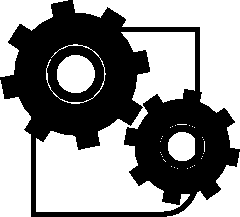
\includegraphics[width=0.75cm]{col11305.imgs/summary_simulation.png} &   \end{array} $ \hspace{2 pt}\raisebox{-5 pt}{} {(section shortcode: P10060 )} \par 
      \label{m38726*uid9}
            \subsection*{The law of conservation of mass}
            \nopagebreak
        \label{m38726*id63198}In order to balance a chemical equation, it is important to understand the law of conservation of mass.\par 
\label{m38726*fhsst!!!underscore!!!id145}
\Definition{  The law of conservation of mass } { The mass of a closed system of substances will remain constant, regardless of the processes acting inside the system. Matter can change form, but cannot be created or destroyed.  } 
        \label{m38726*id63221}For any chemical equation (in a closed system) the \textbf{mass} of the reactants must be equal to the mass of the products. In order to make sure that this is the case, the number of \textbf{atoms} of each element in the reactants must be equal to the number of atoms of those same elements in the products. An example is shown below:\par 
\Tip{Iron is a metal. When we represent it in a balanced chemical equation, we write only $\text{Fe}$. Sulphur occurs as $\text{S}_{8}$ but we write only the empirical formula: $\text{S}$. We do this for all network structures. Writing formulae like this represents \textsl{one unit} of the compound or network structure.}
\begin{table}[H]
\begin{center}
\begin{tabular}{|p{3cm}p{3cm}|p{3cm}|}\hline
\scalebox{.4}{
\begin{pspicture}(0,0)(15,15)
\rput(0,0.5){\psframe(0,0)(3,2)
\rput(0.1,0){\multirput(0.2,0.2)(0.4,0){7}{\pscircle(0,0){0.2}}
\multirput(0.4,0.55)(0.4,0){6}{\pscircle(0,0){0.2}}
\multirput(0.2,0.9)(0.4,0){7}{\pscircle(0,0){0.2}}}}
\end{pspicture}} & 
\scalebox{.4}{
\begin{pspicture}(0,0)(15,15)
\rput(0,0.5){\psframe(0,0)(3,2)
\rput(0.1,0){\multirput(0.2,0.2)(0.4,0){7}{\pscircle[fillstyle=solid,fillcolor=gray](0,0){0.2}}
\multirput(0.4,0.55)(0.4,0){6}{\pscircle[fillstyle=solid,fillcolor=gray](0,0){0.2}}
\multirput(0.2,0.9)(0.4,0){7}{\pscircle[fillstyle=solid,fillcolor=gray](0,0){0.2}}}}
\end{pspicture}} & 
\scalebox{.4}{
\begin{pspicture}(0,0)(15,15)
\rput(0,0.5){\psframe(0,0)(3,2)
\rput(0.1,0){\multirput(0.2,0.2)(0.4,0){7}{\pscircle[fillstyle=solid,fillcolor=gray](0,0){0.2}}
\multirput(0.4,0.55)(0.4,0){6}{\pscircle(0,0){0.2}}
\multirput(0.2,0.9)(0.4,0){7}{\pscircle[fillstyle=solid,fillcolor=gray](0,0){0.2}}}}
\end{pspicture}} \\ \hline
\multicolumn{3}{|c|}{$\text{Fe} + \text{S} \to \text{FeS}$} \\ \hline
Mass of one atom of $\text{Fe}$ is $55,8$ & Mass of one atom of $\text{S}$ is $32,1$ & Mass of one atom of $\text{FeS}$ is $87,9$  \\ \hline
\multicolumn{2}{|c|}{Mass of reactants is $87,9$} & Mass of products is $87,9$ \\ \hline
\end{tabular}
\end{center}
\label{tab:conservmass}
\end{table}

To calculate the \textbf{mass of the molecules} we use the relative atomic masses for iron and sulphur, as seen in table~\ref{tab:conservmass}. You will notice that the mass of the reactants equals the mass of the product. A chemical equation that is \textbf{balanced} will always reflect the \textbf{law of conservation of mass} and the \textbf{law of conservation of atoms}.  
      \label{m38726*eip-619}
            \begin{activity}{Balancing chemical equations}
            \nopagebreak 
% \begin{minipage}{\textwidth}
% \begin{enumerate}[label=\textbf{\arabic*}]
% \item
 \textbf{1.}           \label{m38726*eip-695}You will need: coloured balls (or marbles), prestik, a sheet of paper and coloured pens.
\par 
\label{m38726*eip-69823}We will try to balance the following equation:
\label{m38726*eid0342}\nopagebreak\noindent{}
    \begin{equation*}
    \text{Al}+{\text{O}}_{2}\to {\text{Al}}_{2}{\text{O}}_{3}
      \end{equation*}
Take one ball of one colour. This represents a molecule of $\text{Al}$. Take two balls of another colour and stick them together. This represents a molecule of ${\text{O}}_{2}$. Place these molecules on your left. Now take two balls of the first colour and three balls of the second colour to form ${\text{Al}}_{2}{\text{O}}_{3}$. Place this compound on your right. On a piece of paper draw coloured circles to represent the balls. Draw a line down the centre of the paper to represent the molecules on the left and on the right. 
\par 
\label{m38726*id23534}
Count the number of balls on the left and the number on the right. Do you have the same number of each colour on both sides? If not, the equation is not balanced. How many balls of each colour will you have to add to each side to make the number of balls the same? How would you add these balls?
\par
\label{m38726*id09873432}You should find that you need four balls of the first colour for $\text{Al}$ and three pairs of balls of the second colour (i.e.\@{} six balls in total) for ${\text{O}}_{2}$ on the left side. On the right side you should find that you need 2 clusters of balls for ${\text{Al}}_{2}{\text{O}}_{3}$.
We say that the balanced equation is:\\
    $4\text{Al}+3{\text{O}}_{2}\to 2{\text{Al}}_{2}{\text{O}}_{3}$
\textbf{2.} Use jelly tots and toothpicks to build the following chemical equation. Make sure that your atoms are balanced. Use the same colour jelly tots for the same atoms.\\
$\text{C} + {\text{H}}_{2}\text{O} \to {\text{CO}}_{2} + {\text{CO}} + \text{H}_{2}$ \\
Add compounds until the atoms are balanced. Write the equation down and use a coefficient to indicate how many compounds you used. For example if you had to use three water molecules then write $3{\text{H}}_{2}\text{O}$ 
% \end{enumerate}
% \end{minipage}
% \begin{minipage}{\textwidth}
% \begin{enumerate}[label=\textbf{\arabic*}]
% \setcounter{enumi}{2}
\textbf{3} Use ball and stick drawings to balance the atoms in the following reaction: \\
${\text{NH}}_{3} + {\text{O}}_{2} \to {\text{NO}} + \text{H}_{2}\text{O}$ \\
Use your drawings to write a balanced chemical equation for the reaction.

\textbf{4} Lead ($\text{Pb}$), lead (IV) oxide (${\text{PbO}}_{2}$) and sulphuric acid (${\text{H}}_{2}{\text{SO}}_{4}$) are used in car batteries. The following reaction takes place:
$\text{Pb} + \text{PbO}_{2} + \text{H}_{2}\text{SO}_{4} \to {\text{PbSO}}_{4} + {\text{H}}_{2}\text{O}$ \\
Cut out circles from four different colours of paper to represent each
of the atoms. Build a few of the compounds
($\text{Pb}\ \text{PbO}_{2}\ \text{H}_{2}\text{SO}_{4}$).
These are the
reactants. Do not build the products. Rearrange the atoms so that the
products are formed. Add more reactants if needed to balance the atoms
(e.g.\@{} you will need two $\text{H}_{2}\text{SO}_{4}$
molecules). Use what you have learnt to write a balanced equation for
the reaction.
% \end{enumerate}
 \begin{center}
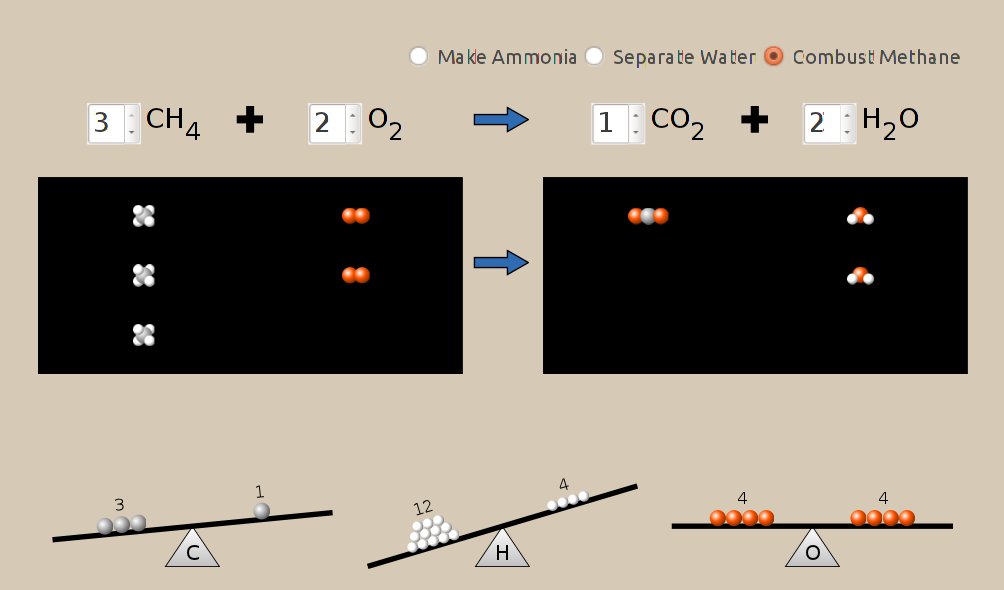
\includegraphics[width=.7\textwidth]{photos/BalancingChemEqu.png}\par
 \end{center}
% \end{minipage}

\end{activity}
\par \label{m38726*uid10}
            \subsection*{Steps to balance a chemical equation through inspection}
            \nopagebreak
        \label{m38726*id63708}When balancing a chemical equation, there are a number of steps that need to be followed. 
\begin{enumerate}[noitemsep, label=\textbf{Step \arabic*}:]
\item Identify the reactants and the products in the reaction and write their chemical formulae.
\item Write the equation by putting the reactants on the left of the arrow and the products on the right.
\item Count the number of atoms of each element in the reactants and the number of atoms of each element in the products.
\item If the equation is not balanced, change the coefficients of the molecules until the number of atoms of each element on either side of the equation balance.
\item Check that the atoms are in fact balanced.
\item (we will look at this a little later): Add any extra details to the equation e.g.\@{} phase symbols.
\end{enumerate}

      \noindent
\begin{wex}{Balancing chemical equations 1}{Balance the following equation:
\begin{center}
${\text{Mg} + \text{HCl} \rightarrow \text{MgCl}_{2} + \text{H}_{2}}$\\
\end{center}
}{\westep{Identify the reactants and products} This has been done in the question.
\westep{Write the equation for the reaction} This has been done in the question.

\westep{Count the number of atoms of each element in the reactants and products}

Reactants: $\text{Mg} = 1 ~\text{atom;}~ \text{H} = 1 ~\text{atom;}~ \text{Cl} = 1 ~\text{atom}$

Products: $\text{Mg} = 1 ~\text{atom;}~ \text{H} = 2 ~\text{atoms;}~ \text{Cl} = 2 ~\text{atoms}$

\westep{Balance the equation}
The equation is not balanced since there are two chlorine atoms in the product and only one in the reactants. If we add a coefficient of two to the HCl to increase the number of H and Cl atoms in the reactants, the equation will look like this:
\begin{center}
${\text{Mg} + 2\text{HCl} \rightarrow \text{MgCl}_{2} + \text{H}_{2}}$\\
\end{center}

\westep{Check that the atoms are balanced}
If we count the atoms on each side of the equation, we find the following:

Reactants: $\text{Mg} = 1;~ \text{H} = 2;~ \text{Cl} = 2$

Products: $\text{Mg} = 1;~ \text{H} = 2;~ \text{Cl} = 2$

The equation is balanced. The final equation is:
\begin{center}
${\text{Mg} + 2\text{HCl} \rightarrow \text{MgCl}_{2} + \text{H}_{2}}$
\end{center}
}
\end{wex}
      \noindent \vspace{-.5cm}
\begin{wex}{Balancing chemical equations 2}{Balance the following equation:
\begin{center}
${\text{CH}_{4} + \text{O}_{2} \rightarrow \text{CO}_{2} + \text{H}_{2}\text{O}}$
\end{center}
}{
% \westep{Identify the reactants and products} This has been done in the question.
% \westep{Write the equation for the reaction} This has been done in the question.
\westep{Count the number of atoms of each element in the reactants and products}

Reactants: $\text{C} = 1;~ \text{H} = 4;~ \text{O} = 2$

Products: $\text{C} = 1;~ \text{H} = 2;~ \text{O} = 3$


\westep{Balance the equation}

If we add a coefficient of 2 to $\text{H}_{2}\text{O}$, then the number of hydrogen atoms in the products will be 4, which is the same as for the reactants. The equation will be:

\begin{center}
${\text{CH}_{4} + \text{O}_{2} \rightarrow \text{CO}_{2} + 2\text{H}_{2}\text{O}}$\\
\end{center}

\westep{Check that the atoms balance}

Reactants: $\text{C} = 1;~ \text{H} = 4;~ \text{O} = 2$

Products: $\text{C} = 1;~ \text{H} = 4; ~\text{O} = 4$

You will see that, although the number of \textit{hydrogen} atoms now balances, there are more oxygen atoms in the products. You now need to repeat the previous step. If we put a coefficient of 2 in front of $\text{O}_{2}$, then we will increase the number of oxygen atoms in the reactants by 2. The new equation is:

\begin{center}
${\text{CH}_{4} + 2\text{O}_{2} \rightarrow \text{CO}_{2} + 2\text{H}_{2}\text{O}}$
\end{center}

When we check the number of atoms again, we find that the number of atoms of each element in the reactants is the same as the number in the products. The equation is now balanced.
}
\end{wex}
      \noindent \vspace{-.5cm}
\begin{wex}{Balancing chemical equations 3}{In our bodies, sugar ${\text{(C}_{6}\text{H}_{12}\text{O}_{6}\text{)}}$ reacts with the oxygen we breathe in to produce carbon dioxide, water and energy. Write the balanced equation for this reaction.}{\westep{Identify the reactants and products in the reaction.}
Reactants: sugar (${\text{C}_{6}\text{H}_{12}\text{O}_{6}}$) and oxygen (${\text{O}_{2}}$)

Products: carbon dioxide (${\text{CO}_{2}}$) and water (${\text{H}_{2}\text{O}}$)\\

\westep{Write the equation}
    $\text{C}_{6}\text{H}_{12}\text{O}_{6} + \text{O}_{2} \rightarrow \text{CO}_{2} + \text{H}_{2}\text{O}$

\westep{Count the number of atoms of each element in the reactants and in the products}
   Reactants: $\text{C} = 6;~ \text{H} = 12; ~\text{O} = 8$

   Products: $\text{C} = 1;~ \text{H} = 2; ~\text{O} = 3$

\westep{Balance the equation}
   It is easier to start with carbon as it only appears once on each side. If we add a $6$ in front of ${\text{CO}_{2}}$, the equation looks like this:\\
    $\text{C}_{6}\text{H}_{12}\text{O}_{6} + \text{O}_{2} \rightarrow 6\text{CO}_{2} + \text{H}_{2}\text{O}$\\

   Reactants: $\text{C} = 6;~ \text{H} = 12; ~\text{O} = 8$

   Products: $\text{C} = 6;~ \text{H} = 2; ~\text{O} = 13$

\westep{Change the coefficients again to try to balance the equation.}
Let us try to get the number of hydrogens the same this time.\\
    $\text{C}_{6}\text{H}_{12}\text{O}_{6} + \text{O}_{2} \rightarrow 6\text{CO}_{2} + 6\text{H}_{2}\text{O}$

   Reactants: $\text{C} = 6;~ \text{H} = 12; ~\text{O} = 8$

   Products: $\text{C} = 6;~ \text{H} = 12; ~\text{O} = 18$

\westep{Now we just need to balance the oxygen atoms.}
  $\text{C}_{6}\text{H}_{12}\text{O}_{6} + 6\text{O}_{2} \rightarrow 6\text{CO}_{2} + 6\text{H}_{2}\text{O}$

   Reactants: $\text{C} = 6;~ \text{H} = 12; ~\text{O} = 18$

   Products: $\text{C} = 6;~ \text{H} = 12; ~\text{O} = 18$
}
\end{wex}
    \noindent
\simulation{PhET simulation for balancing equations}{VPeea}
\vspace{.5cm}
            \begin{exercises}{ Balancing simple chemical equations }
            \nopagebreak \noindent 
 \label{m38726*id65193}Balance the following equations:
 \label{m38726*id65199}\begin{enumerate}[noitemsep, label=\textbf{\arabic*}. ] 
%Question 1
\item  $\text{Mg} + \text{O}_{2} \to \text{MgO}$
%Q2
\item ${\text{Ca}}+{\text{H}}_{2}\text{O} \to \text{Ca(OH)}_{2} + \text{H}_{2}$
%Q3
\item ${\text{CuCO}}_{3} + {\text{H}}_{2}{\text{SO}}_{4} \to \text{CuSO}_{4} + {\text{H}}_{2}\text{O} + {\text{CO}}_{2}$
%Q4
\item $\text{CaCl}_{2} + {\text{Na}}_{2}{\text{CO}}_{3} \to \text{CaCO}_{3} + {\text{NaCl}}$        
%Q5
\item ${\text{C}}_{12}{\text{H}}_{22}{\text{O}}_{11} + \text{O}_{2} \to \text{H}_{2}\text{O} + \text{CO}_{2}$
%Q6
\item Barium chloride reacts with sulphuric acid to produce barium sulphate and hydrochloric acid.
%Q7
\item Ethane (${\text{C}}_{2}{\text{H}}_{6}$) reacts with oxygen to form carbon dioxide and steam.
%Q8
\item Ammonium carbonate is often used as a smelling salt. Balance the following reaction for the decomposition of ammonium carbonate: ${\text{(NH}}_{4}\text{)}_{2}{\text{CO}}_{3} \text{(s)} \to {\text{NH}}_{3}\text{(aq)} + {\text{CO}}_{2} \text{(g)} + \text{H}_{2}\text{O} (\ell)$ 
%Q9
\item Hydrogen fuel cells are extremely important in the development of alternative energy sources. Many of these cells work by reacting hydrogen and oxygen gases together to form water, a reaction which also produces electricity. Balance the following equation: $\text{H}_{2} \text{(g)} + \text{O}_{2} \text{(g)} \to \text{H}_{2}\text{O} (\ell)$    
%Q10
\item The synthesis of ammonia ($\text{NH}_{3}$), made famous by the German chemist Fritz Haber in the early 20th century, is one of the most important reactions in the chemical industry. Balance the following equation used to produce ammonia:
$\text{N}_{2} \text{(g)} + \text{H}_{2} \text{(g)} \to \text{NH}_{3} \text{(g)}$
\end{enumerate} 
\practiceinfo
\begin{tabular}[h]{cccccc}
 (1.) 005g  &  (2.) 005h   &  (3.) 005i  &  (4.) 005j  &  (5.) 005k  &  (6.) 005m  &  (7.) 005n  &  (8.) 005p  &  (9.) 005q  &  (10.) 005r  & \end{tabular}
\end{exercises}
         \subsection*{State symbols and other information}
    \nopagebreak
%            \label{m38727} $ \hspace{-5pt}\begin{array}{cccccccccccc}   
\includegraphics[width=0.75cm]{col11305.imgs/summary_fullmarks.png} &   
\includegraphics[width=0.75cm]{col11305.imgs/summary_video.png} &   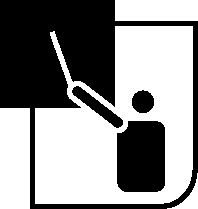
\includegraphics[width=0.75cm]{col11305.imgs/summary_presentation.png} &   \end{array} $ \hspace{2 pt}\raisebox{-5 pt}{} {(section shortcode: P10061 )} \par 
      \label{m38727*id65920}The state (phase) of compounds can be expressed in the chemical equation. This is done by placing the correct label on the right hand side of the formula. The following four labels can be used:\par \noindent 
      \label{m38727*id65925}\begin{enumerate}[noitemsep, label=\textbf{\arabic*}.] 
\item (g) for gaseous compounds
\label{m38727*uid28}\item ($\ell$) for liquids
\label{m38727*uid29}\item (s) for solid compounds
\label{m38727*uid30}\item (aq) for an aqueous (water) solution
\end{enumerate}
\label{m38727*eip-536}To show that heat is needed for a reaction, a Greek delta ($\Delta $) is placed above the arrow. For example: $\text{NH}_{4}\text{Cl} \xrightarrow{\Delta} \text{NH}_{3} + \text{HCl}$ 
\vspace{-.5cm}
\label{m38727*secfhsst!!!underscore!!!id967} 
      \noindent
\begin{wex}{Balancing chemical equations 4}{Solid zinc metal reacts with aqueous hydrochloric acid to form an aqueous solution of zinc chloride ($\text{ZnCl}_{2}$) and hydrogen gas. Write a balanced equation for this reaction.}{\westep{Identify the reactants and products}
The reactants are zinc ($\text{Zn}$) and hydrochloric acid ($\text{HCl}$). The products are zinc chloride ($\text{ZnCl}_{2}$) and hydrogen ($\text{H}_{2}$).

\westep{Write the equation}
${\text{Zn} + \text{HCl} \rightarrow \text{ZnCl}_{2} + \text{H}_{2}}$

\westep{Balance the equation}
You will notice that the zinc atoms balance but the chlorine and hydrogen atoms do not. Since there are two chlorine atoms on the right and only one on the left, we will give HCl a coefficient of 2 so that there will be two chlorine atoms on each side of the equation.\\
${\text{Zn} + 2\text{HCl} \rightarrow \text{ZnCl}_{2} + \text{H}_{2}}$

\westep{Check that all the atoms balance}
When you look at the equation again, you will see that all the atoms are now balanced.

\westep{Ensure all details (e.g.\@{} state symbols) are added}
In the initial description, you were told that zinc was a metal, hydrochloric acid and zinc chloride were in aqueous solutions and hydrogen was a gas.\\
$\text{Zn (s)} + \text{HCl (aq)} \rightarrow \text{ZnCl}_{2} \text{(aq)} + \text{H}_{2} \text{(g)}$
}
\end{wex}
    \noindent
\mindsetvid{Khan academy video on balancing equations}{VPemn}
\begin{exercises}{State symbols}
            \nopagebreak \vspace{-1cm}
      \label{m38727*id66790}Write balanced equations for each of the following reactions, include state symbols:\par 
      \label{m38727*id66796}\begin{enumerate}[noitemsep, label=\textbf{\arabic*}. ] 
%Q1
        \label{m38727*uid33}\item Lead (II) nitrate solution reacts with a potassium iodide solution to form a precipitate (solid) of lead iodide while potassium nitrate remains in solution.
%Q2
\label{m38727*uid34}\item When heated, aluminium metal reacts with solid copper oxide to produce copper metal and aluminium oxide (${\text{Al}}_{2}{\text{O}}_{3}$).
%Q3
\label{m38727*uid35}\item When calcium chloride solution is mixed with silver nitrate solution, a white precipitate (solid) of silver chloride appears. Calcium nitrate ($\text{Ca(NO}_{3}\text{)}_{2}$) is also produced in the solution.
%Q4
\item Solid ammonium carbonate decomposes to form three gaseous products.
        \end{enumerate}
\practiceinfo
 \begin{tabular}[h]{cccccc}
 (1.) 00b7&  (2.) 00b8&  (3.) 00b9&  (4.) 00ba&    &   &   &   &   &   & \end{tabular}
\end{exercises}
\vspace{-1cm}
\begin{g_experiment}{The relationship between product and reactant}
\textbf{Aim:} To investigate the relationship between the amount of product and the amount of reactant.\\
\textbf{Apparatus:}\\
\begin{minipage}{.5\textwidth}
 \begin{itemize}[noitemsep]
  \item flask
\item measuring cylinder
\item water bowl
\item delivery tube
\item funnel with stopcock
\item stopper
\item sodium hydrogen carbonate ($\text{NaHCO}_{3}$) powder
\item dilute sulphuric acid ($\text{H}_{2}\text{SO}_{4}$)
 \end{itemize}
\end{minipage}
\begin{minipage}{.5\textwidth}
\begin{center}
\scalebox{0.8}{
 \begin{pspicture}(0,0)(5,5)
\psset{unit=0.5cm,glassType=erlen}
\newpsstyle{white} {linestyle=solid,linecolor=black,linewidth=.1,fillstyle=solid,fillcolor=white}
 \pstChauffageBallon[recuperationGaz,doubletube,aspectLiquide1=white,niveauLiquide1=20]
\end{pspicture}
}
\end{center}
\end{minipage} \\
\textbf{Method:} 
\begin{enumerate}[noitemsep,label=\textbf{\arabic*}]
 \item Weigh $20~\text{g}$ of $\text{NaHCO}_{3}$ and place it into a flask.
\item Set up the above apparatus.
\item Measure out $5~\text{ml}$ of $\text{H}_{2}\text{SO}_{4}$ and carefully pour this into the funnel (make sure that the stopcock is closed).
\item Slowly add the $\text{H}_{2}\text{SO}_{4}$ to the $\text{NaHCO}_{3}$ by opening the stopcock.
\item Observe what happens.
\item Record the volume of gas collected in the measuring cylinder.
\item Repeat the above steps but this time use $10~\text{ml}$ of $\text{H}_{2}\text{SO}_{4}$.
\item Write a balanced equation for this reaction. (Hint: carbon dioxide gas is formed, as well as water and sodium sulphate.)
\end{enumerate}
\textbf{Results and discussion: } You should observe that more gas is formed when using more $\text{H}_{2}\text{SO}_{4}$. 
\end{g_experiment}

%     \label{m38727*eip-429}Balanced equations are very important in chemistry. It is only by working with balanced equations that chemists can perform many different calculations that tell them what quantity of something reacts. In a later chapter we will learn how to work with some of these calculations. We can interpret balanced chemical equations in terms of the conservation of matter, the conservation of mass or the conservation of energy. 
% \label{m38727*eip-366}
%     \setcounter{subfigure}{0}
% 	\begin{figure}[H] % horizontal\label{m38727*slidesharefigure}
%     \label{m38727*slidesharemedia}\label{m38727*slideshareflash}\raisebox{-5 pt}{ 
\includegraphics[width=0.5cm]{col11305.imgs/summary_www.png}} { (Presentation:  P10063 )} \end{figure}
\summary{VPeca}
            \nopagebreak
      \label{m38727*id67171}\begin{itemize}[noitemsep]
            \label{m38727*uid36}\item A \textbf{chemical equation} uses symbols to describe a chemical reaction.
\label{m38727*uid37}\item In a chemical equation, \textbf{reactants} are written on the left hand side of the equation and the \textbf{products} on the right. The arrow is used to show the direction of the reaction.
\label{m38727*uid38}\item When representing chemical change, it is important to be able to write the \textbf{chemical formula} of a compound.
\item The law of conservation of mass states that the mass of a closed system of substances will remain constant, regardless of the processes acting inside the system. Matter can change form, but cannot be created or destroyed.
\label{m38727*uid39}\item In any chemical reaction, the \textbf{law of conservation of mass} applies. This means that the total atomic mass of the reactants must be the same as the total atomic mass of the products. This also means that the total number of atoms of the reactants must be the same as the total number of atoms of the product.
\label{m38727*uid40}\item If the number of atoms of each element in the reactants is the same as the number of atoms of each element in the product, then the equation is \textbf{balanced}.
\label{m38727*uid41}\item If the number of atoms of each element in the reactants is not the same as the number of atoms of each element in the product, then the equation is \textbf{not balanced}.
\label{m38727*uid42}\item In order to balance an equation, \textbf{coefficients} can be placed in front of the reactants and products until the number of atoms of each element is the same on both sides of the equation.
\item The state of the compounds in a chemical reaction can be expressed in the chemical equation by using one of four symbols. The symbols are g (gas), $\ell$ (liquid), s (solid) and aq (aqueous solutions). These symbols are written in brackets after the compound.
\end{itemize}
\label{m38727*secfhsst!!!underscore!!!id1434}
            \begin{eocexercises}{Representing chemical change}
            \nopagebreak \noindent \vspace{-.5cm}
      \label{m38727*id67334}\begin{enumerate}[noitemsep, label=\textbf{\arabic*}. ] 
%Q1
\label{m38727*uid45}\item Propane is a fuel that is commonly used as a heat source for engines and homes. Balance the following equation for the combustion of propane:
${\text{C}}_{3}{\text{H}}_{8} (\ell) + \text{O}_{2} \text{(g)} \to \text{CO}_{2} \text{(g)} + \text{H}_{2}\text{O} (\ell)$
%Q2
        \label{m38727*uid47}\item Methane ($\text{CH}_{4}$) burns in oxygen according to the following reaction. \\
\begin{figure}[H]
\begin{center}
 \includegraphics[width=.8\textwidth]{photos/methane_O2_rxn.png}
\end{center}
\end{figure}
\begin{enumerate}[noitemsep, label=\textbf{\alph*}.]
 \item Complete the diagrams by drawing ball-and-stick models of the products.
\item Write a balanced chemical equation for the reaction and include state symbols.
\end{enumerate}
%Q3
 \label{m38727*uid48}\item Chemical weapons were banned by the Geneva Protocol in 1925. According to this protocol, all chemicals that release suffocating and poisonous gases are not to be used as weapons. White phosphorus, a very reactive allotrope of phosphorus, was recently used during a military attack. Phosphorus burns vigorously in oxygen. Many people got severe burns and some died as a result. The equation for this spontaneous reaction is:
        ${\text{P}}_{4}\left(\text{s}\right)+{\text{O}}_{2}\left(\text{g}\right)\to {\text{P}}_{2}{\text{O}}_{5}\left(\text{s}\right)$\label{m38727*id67821}\begin{enumerate}[noitemsep, label=\textbf{\alph*}. ] 
            \label{m38727*uid49}\item Balance the chemical equation.
\label{m38727*uid50}\item Prove that the law of conservation of mass is obeyed during this chemical reaction.
\label{m38727*uid51}\item Name the product formed during this reaction.
% \label{m38727*uid52}\item Classify the reaction as endothermic or exothermic. Give a reason for your answer.
\label{m38727*uid53}\item Classify the reaction as a synthesis or decomposition reaction. Give a reason for your answer.
        \end{enumerate}
% (DoE Exemplar Paper 2 2007)
%Q4
\item The following diagrams represent the combustion of ethane ($\text{C}_2\text{H}_6$). Complete the diagrams and write a balanced equation for the reaction. Indicate the state symbols. \\
\scalebox{.8} % Change this value to rescale the drawing.
{
\begin{pspicture}(0,-2.015)(10.04,2.015)
\definecolor{color6b}{rgb}{0.5882352941176471,0.5882352941176471,0.5882352941176471}
\definecolor{color7b}{rgb}{0.19607843137254902,0.19607843137254902,0.19607843137254902}
\psframe[linewidth=0.04,dimen=outer](3.98,2.005)(0.0,-1.975)
\psframe[linewidth=0.04,dimen=outer](10.04,2.015)(6.01,-2.015)
\rput{-32.038597}(0.25529027,1.656808){\pscircle[linewidth=0.04,linecolor=color6b,dimen=outer,fillstyle=solid,fillcolor=color6b](3.012965,0.3838178){0.24}}
\rput{-32.038597}(0.44232956,1.8115258){\pscircle[linewidth=0.04,linecolor=color6b,dimen=outer,fillstyle=solid,fillcolor=color6b](3.3759246,0.13544907){0.24}}
\pscircle[linewidth=0.04,linecolor=color7b,dimen=outer,fillstyle=solid,fillcolor=color7b](2.87,-0.735){0.24}
\pscircle[linewidth=0.04,dimen=outer](2.85,-0.385){0.12}
\pscircle[linewidth=0.04,linecolor=color7b,dimen=outer,fillstyle=solid,fillcolor=color7b](3.33,-0.735){0.24}
\pscircle[linewidth=0.04,dimen=outer](2.53,-0.745){0.12}
\pscircle[linewidth=0.04,dimen=outer](2.85,-1.085){0.12}
\pscircle[linewidth=0.04,dimen=outer](3.35,-1.085){0.12}
\pscircle[linewidth=0.04,dimen=outer](3.67,-0.745){0.12}
\pscircle[linewidth=0.04,dimen=outer](3.33,-0.385){0.12}
\pscircle[linewidth=0.04,linecolor=color6b,dimen=outer,fillstyle=solid,fillcolor=color6b](2.82,1.265){0.24}
\pscircle[linewidth=0.04,linecolor=color6b,dimen=outer,fillstyle=solid,fillcolor=color6b](3.26,1.265){0.24}
\rput{32.43465}(-0.57426614,-0.9315801){\pscircle[linewidth=0.04,linecolor=color6b,dimen=outer,fillstyle=solid,fillcolor=color6b](1.3143191,-1.4529942){0.24}}
\rput{32.43465}(-0.38976568,-1.0939419){\pscircle[linewidth=0.04,linecolor=color6b,dimen=outer,fillstyle=solid,fillcolor=color6b](1.6856809,-1.2170057){0.24}}
\rput{-95.96166}(2.008164,2.2169962){\pscircle[linewidth=0.04,linecolor=color6b,dimen=outer,fillstyle=solid,fillcolor=color6b](2.0028498,0.20381016){0.24}}
\rput{-95.96166}(2.3929713,1.6884707){\pscircle[linewidth=0.04,linecolor=color6b,dimen=outer,fillstyle=solid,fillcolor=color6b](1.9571501,-0.23381016){0.24}}
\pscircle[linewidth=0.04,linecolor=color6b,dimen=outer,fillstyle=solid,fillcolor=color6b](2.4,-1.615){0.24}
\pscircle[linewidth=0.04,linecolor=color6b,dimen=outer,fillstyle=solid,fillcolor=color6b](2.84,-1.615){0.24}
\pscircle[linewidth=0.04,linecolor=color6b,dimen=outer,fillstyle=solid,fillcolor=color6b](0.64,0.225){0.24}
\pscircle[linewidth=0.04,linecolor=color6b,dimen=outer,fillstyle=solid,fillcolor=color6b](1.08,0.225){0.24}
\rput{158.27188}(1.526796,-1.8859106){\pscircle[linewidth=0.04,linecolor=color6b,dimen=outer,fillstyle=solid,fillcolor=color6b](0.9443692,-0.7964446){0.24}}
\rput{158.27188}(0.7986616,-1.4203893){\pscircle[linewidth=0.04,linecolor=color6b,dimen=outer,fillstyle=solid,fillcolor=color6b](0.53563076,-0.6335554){0.24}}
\pscircle[linewidth=0.04,linecolor=color7b,dimen=outer,fillstyle=solid,fillcolor=color7b](0.81,1.325){0.24}
\pscircle[linewidth=0.04,dimen=outer](0.79,1.675){0.12}
\pscircle[linewidth=0.04,linecolor=color7b,dimen=outer,fillstyle=solid,fillcolor=color7b](1.27,1.325){0.24}
\pscircle[linewidth=0.04,dimen=outer](0.47,1.315){0.12}
\pscircle[linewidth=0.04,dimen=outer](0.79,0.975){0.12}
\pscircle[linewidth=0.04,dimen=outer](1.29,0.975){0.12}
\pscircle[linewidth=0.04,dimen=outer](1.61,1.315){0.12}
\pscircle[linewidth=0.04,dimen=outer](1.27,1.675){0.12}
\psline[linewidth=0.04cm,arrowsize=0.05291667cm 3.0,arrowlength=1.4,arrowinset=0.0]{->}(4.18,0.045)(5.64,0.025)
\end{pspicture} 
}
%Q5
\item Balance the following chemical equation:\\
${\text{N}}_{2}{\text{O}}_{5}\to {\text{NO}}_{2}+{\text{O}}_{2}$ \\
Draw submicroscopic diagrams to represent this reaction.
%Q6
        \item Sulphur can be produced by the Claus process. This two-step process involves reacting hydrogen sulphide with oxygen and then reacting the sulphur dioxide that is produced with more hydrogen sulphide. The equations for these two reactions are:
\label{m38727*id6243}\nopagebreak\noindent{}
    \begin{eqnarray*}
{\text{H}}_{2}\text{S} + {\text{O}}_{2} \to {\text{SO}}_{2} + {\text{H}}_{2}\text{O} \\ 
{\text{H}}_{2}\text{S} + {\text{SO}}_{2} \to \text{S} + {\text{H}}_{2}\text{O} 
      \end{eqnarray*}
Balance these two equations.
%Q7
\label{m38727*uid46}\item Aspartame, an artificial sweetener, has the formula ${\text{C}}_{14}{\text{H}}_{18}{\text{N}}_{2}{\text{O}}_{2}$. Write the balanced equation for its combustion (reaction with ${\text{O}}_{2}$) to form ${\text{CO}}_{2}$ gas, liquid $\text{H}_{2}\text{O}$, and ${\text{N}}_{2}$ gas.
\end{enumerate} \vspace{-.5cm}
\practiceinfo
 \begin{tabular}[h]{cccccc}
 (1.) 005s  &  (2.) 005t  &  (3.) 005u  &  (4.) 005v  &  (5.) 005w  &  (6.) 005x  &  (7.) 005y  & \end{tabular}
\end{eocexercises}
